\chapter{Dienste}
\label{cha:dienste}
Die Dienstübersicht zeigt alle zukünftigen Dienste absteigend sortiert nach Datum. Jeder Dienst wird als Block klar getrennt und übersichtlich dargestellt. In Abbildung \ref{fig:view_service} \textit{\nameref{fig:view_service}} ist ein einzelner Dienst exemplarisch abgebildet.

\begin{figure}[h]
 \begin{addmargin}{-0.2\linewidth}
   \centering 
   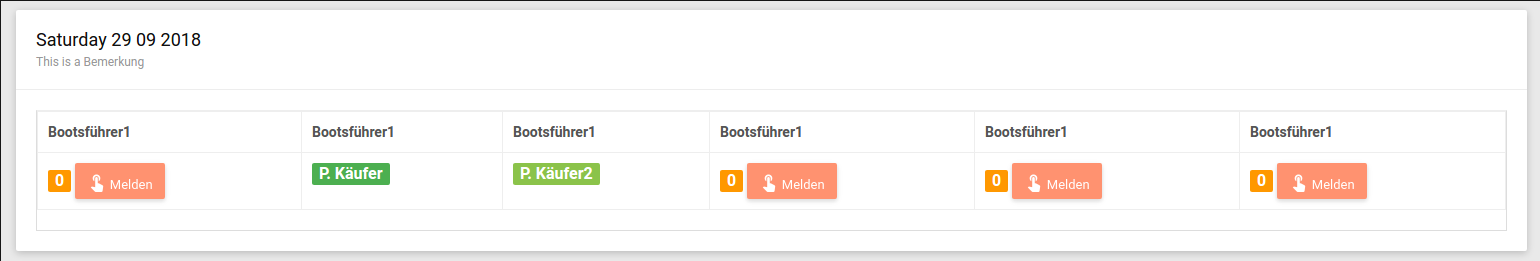
\includegraphics[width=20cm]{Bilder/view_service.png}
 \end{addmargin} 
 \caption[Dienste Übersicht]{DLRG Dienstplan Dienste Übersicht}
 \label{fig:view_service}
\end{figure}

\noindent Jeder Dienst ist mit Tag und Datum beschriftet. Darunter kann eine Bemerkung bzw. Beschreibung hinterlegt sein. Die einzelnen Positionen des Dienstes werden als Tabelle dargestellt.
\noindent Dem Benutzer kann eine Position in fünf verschiedenen Ansichten präsentiert werden mit welchen er zum teil Interagieren kann.
Diese sind in der folgenden Tabelle aufgezeigt. Beispiele beziehen sich immer auf die Abbildung \ref{fig:view_service} \textit{\nameref{fig:view_service}}

\begin{itemize}
\item Melden (bsp. Position 4): Diese Position ist noch nicht zugeteilt. Der Benutzer kann sich hierzu melden.
\item Melden deaktiviert (bsp. Position 1): Diese Position ist noch nicht zugeteilt. Der Benutzer hat aber nicht die entsprechende Qualifikation und kann sich somit für die Position nicht melden.
\item Position bestätigt (bsp. Position 2): Die Position ist bereits zugeteilt.
\item Position bestätigt (bsp. Position 3): Diese Position ist an den Benutzer zugeordnet. Alle zugeordneten Positionen des eigenen Benutzers werden zur besseren Übersicht hellgrün dargestellt.
\item Für Position gemeldet, noch nicht bestätigt (bsp. Position 5): Für diese Position hat der Benutzer sich bereits gemeldet. Solange dies durch die Administratoren noch nicht bestätigt ist, kann die Meldung zurück gezogen werden.
\end{itemize}

\noindent Die in den orangenen Kästen dargestellten Zahlen stehen für die Anzahl an bereits gemeldeten Benutzern für diese Position. Ein Benutzer kann sich für beliebig viele Positionen eines Dienstes melden. Ebenso können beliebig viele Benutzer sich für eine Position melden. Durch die Administratoren wird nur einer Benutzer für eine Position bestätigt.

\noindent Positionen können Kommentare beinhalten (bsp. Position 1). Mit Kommentaren können geteilte Positionen (Position 1 nur bis 14 Uhr) realisiert werden. Des weiteren können mit Kommentaren auch auf Besonderheiten zu dieser Position hingewiesen werden.


\section{Mobile Ansicht}
\label{sec:dienste_mobile}
Die GUI auf Mobilgeräten, wie \zB Smartphones oder Tablets, weicht von der Desktopversion leicht ab. Die einzelnen Dienste sind eingeklappt und können mit einem Tippen auf den kleinen Pfeil oder das Datum ausgeklappt werden (\ref{fig:view_service_mobile_close} \textit{\nameref{fig:view_service_mobile_close}}). 


\begin{figure}[h]
 \begin{addmargin}{-0.2\linewidth}
   \centering 
   
\includegraphics[width=20cm]{Bilder/view_service_mobile_close.png}
 \end{addmargin} 
 \caption[Dienste Übersicht Mobil]{DLRG Dienstplan Dienste Übersicht Mobil eingeklappt}
 \label{fig:view_service_mobile_close}
\end{figure}


\noindent Die rot hinterlegte Zahl zwischen dem kleinen Pfeil und dem Datum gibt die Anzahl der noch nicht zugewiesenen Positionen eines Dienstes an. Die Berechnung stützt sich hierbei lediglich auf Positionen welche für eine Mindestbesatzung relevant sind. In Abbildung \ref{fig:view_service_mobile} \textit{\nameref{fig:view_service_mobile}} ist die Zahl 6 zu sehen da wie in der ausgeklappten Ansicht zu sehen ist, 6 Positionen noch nicht zugewiesen wurden.

\begin{figure}[h]
 \begin{addmargin}{-0.2\linewidth}
   \centering 
   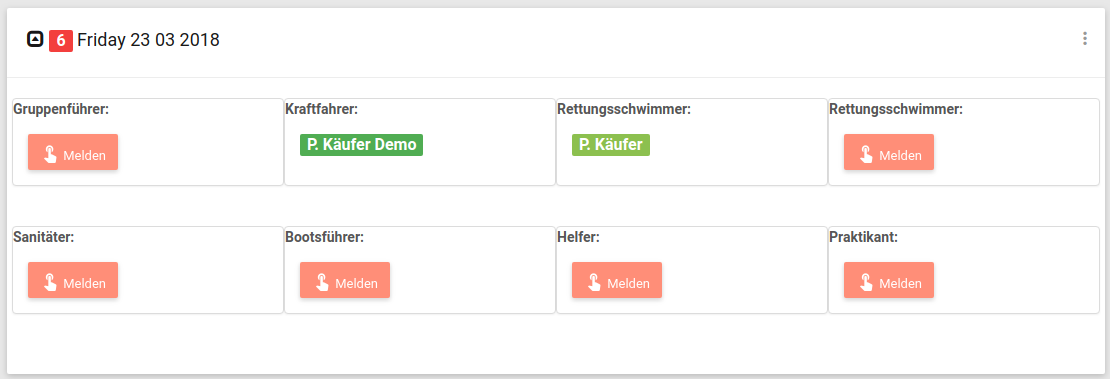
\includegraphics[width=20cm]{Bilder/view_service_mobile.png}
 \end{addmargin} 
 \caption[Dienste Übersicht Mobil Ausgeklappt]{DLRG Dienstplan Dienste Übersicht Mobil ausgeklappt}
 \label{fig:view_service_mobile}
\end{figure}